\section{Coexistence Scenarios}

\todo{rewrite this section if necessary}

The previous section investigated the borders where stable cycles disappear.
We can see that parameter regions where only one stable cycle exists (``Type A'') can overlap.
For example, the upper border where the cycle $\Cycle{\A^5\B^3\C^5\D^3}$ disappears, marked blue in \Cref{fig:final.regions.E.halved}, is above the lower border where the stable cycle $\Cycle{\A^4\B^3\C^4\D^3}$ disappears, marked red.
This means that there is a coexistence of the cycles in the overlapping parameter region, marked with the point $M$.
This section will take a look at all possible coexistence scenarios of cycles starting with the simplest case, a single ``Type A'' parameter region.

\begin{figure}
    \centering
    \begin{subfigure}{0.4\textwidth}
        \centering
        \includegraphics[width=\textwidth]{60_MinimalRepr/2D_Regions_E/result.png}
        \caption{Showing $E_{16}$}
        \label{fig:final.regions.E.halved}
    \end{subfigure}
    \begin{subfigure}{0.4\textwidth}
        \centering
        \includegraphics[width=\textwidth]{60_MinimalRepr/2D_Regions_F/result.png}
        \caption{Showing $F_{16}$}
        \label{fig:final.regions.F.halved}
    \end{subfigure}
    \caption{2D Period Regions of Halved Final Model Showing a ``Type A'' and a ``Type B'' Region}
\end{figure}

\subsection{Only One ``Type A'' Parameter Region}

As mentioned above, the simplest case of coexistence in this model is the existence of a stable cycle of a ``Type A'' parameter region on its own.
A point where this is the case is the point $L$ in \Cref{fig:final.regions.E.halved}.
Here there is only one stable cycle, $\Cycle{\A^5\B^3\C^5\D^3}$.

\todo{pic, describe, color?}

\subsection{Two ``Type A'' Parameter Regions Overlapping}
\label{sec:minrep.coex.AA}

``Type A'' parameter regions can overlap with one another.
This can happen in four different ways.
Assuming the stable cycle of the parameter region in the middle is $\Cycle{\A^x\B^y\C^x\D^y}$, it can overlap with parameter regions, where either one of the following cycles is stable
\begin{enumerate*}
    \item $\Cycle{\A^{x-1}\B^y\C^{x-1}\D^y}$,
    \item $\Cycle{\A^x\B^{y+1}\C^x\D^{y+1}}$,
    \item $\Cycle{\A^{x+1}\B^y\C^{x+1}\D^y}$, and
    \item $\Cycle{\A^x\B^{y-1}\C^x\D^{y-1}}$.
\end{enumerate*}
For the concrete case pictured in \Cref{fig:final.regions.E.halved}, this results in the following parameter regions
\begin{enumerate}
    \item $\P_{\A^5\B^3\C^5\D^3, \A^4\B^3\C^4\D^3}$ marked with $M$,
    \item $\P_{\A^5\B^3\C^5\D^3, \A^5\B^4\C^5\D^4}$ marked with $N$,
    \item $\P_{\A^5\B^3\C^5\D^3, \A^6\B^3\C^6\D^3}$ marked with $O$, and
    \item $\P_{\A^5\B^3\C^5\D^3, \A^5\B^2\C^5\D^2}$ marked with $P$.
\end{enumerate}
\Cref{fig:minrep.cobweb.M} shows the cobweb diagram for the parameter values at point $M$.
Here we can see the two cycles of the two different ``type A'' parameter regions.
The cycle $\Cycle{\A^5\B^3\C^5\D^3}$ is blue and the cycle $\Cycle{\A^4\B^3\C^4\D^3}$ is red, these colors will stay the same for other cobweb diagrams in this section.
The cobweb diagram also shows the basins of attraction of both cycles, blue for the cycle $\Cycle{\A^5\B^3\C^5\D^3}$ and red for the cycle $\Cycle{\A^4\B^3\C^4\D^3}$.

\begin{figure}
    \centering
    \subfloat[Two ``type A'' parameter regions overlapping at point $M$]{
        \includegraphics[width=.45 \textwidth]{60_MinimalRepr/Cobweb_M/Manual/result.png}
        \label{fig:minrep.cobweb.M}
    }
    \subfloat[Only a ``type B'' parameter region at point $Q$]{
        \includegraphics[width=.45 \textwidth]{60_MinimalRepr/Cobweb_Q/Manual/result.png}
        \label{fig:minrep.cobweb.Q}
    }
    \caption{Cobwebs for scenarios of 2 coexisting cycles}
\end{figure}

\subsection{Only one ``Type B'' Parameter Region}

Another very simple case is when a ``Type B'' parameter region does not overlap with any other region.
In this case, there are two coexisting stable cycles as discussed before in \Cref{sec:og.dynamics} and \Cref{sec:minrep.dynamics}.
Here the cycles are asymmetrical if one of the cycles is $\Cycle{\A^x\B^y\C^{x-1}\D^{y+1}}$, the other cycle is $\Cycle{\A^{x-1}\B^{y+1}\C^x\D^y}$.
In the concrete case marked in \Cref{fig:final.regions.F.halved} as point $Q$, these cycles are $\Cycle{\A^5\B^3\C^4\D^4}$ and $\Cycle{\A^4\B^4\C^5\D^3}$.

\Cref{fig:minrep.cobweb.Q} show the cobweb diagram for the parameter values at this point.
The cycle $\Cycle{\A^5\B^3\C^4\D^4}$ is green and its rotated twin $\Cycle{\A^4\B^4\C^5\D^3}$ is brown.
Again, for the rest of this section, the colors will stay the same when we encounter these cycles again in cobwebs.
The basins of attraction are shown as well in the corresponding color for each cycle.

\subsection{One ``Type B'' and One ``Type A'' Parameter Region Overlapping}
\label{sec:minrep.coex.BA}

We can see in \Cref{fig:final.regions.F.halved}, that this ``Type B'' parameter region can overlap with ``Type A'' parameter regions.
This can also happen in four different ways, as was the case with ``Type A'' parameter regions overlapping with one another (described in \Cref{sec:minrep.coex.AA}).
Assuming the stable cycles of the parameter region in the middle are $\Cycle{\A^x\B^y\C^{x-1}\D^{y+1}}$ and $\Cycle{\A^{x-1}\B^{y+1}\C^x\D^y}$, it can overlap with parameter regions, where either one of the following cycles is stable
\begin{enumerate*}
    \item $\Cycle{\A^{x-1}\B^{y+1}\C^{x-1}\D^{y+1}}$,
    \item $\Cycle{\A^x\B^{y+1}\C^x\D^{y+1}}$,
    \item $\Cycle{\A^x\B^y\C^x\D^y}$, and
    \item $\Cycle{\A^{x-1}\B^y\C^{x-1}\D^y}$.
\end{enumerate*}
So in these cases, there will be three coexisting stable cycles.
For the concrete case pictured in \Cref{fig:final.regions.F.halved}, this results in the following parameter regions
\begin{enumerate}
    \item $\P_{\A^5\B^3\C^4\D^4, \A^4\B^4\C^5\D^3, \A^4\B^4\C^4\D^4}$ marked with $R$,
    \item $\P_{\A^5\B^3\C^4\D^4, \A^4\B^4\C^5\D^3, \A^5\B^4\C^5\D^4}$ marked with $S$,
    \item $\P_{\A^5\B^3\C^4\D^4, \A^4\B^4\C^5\D^3, \A^5\B^3\C^5\D^3}$ marked with $T$, and
    \item $\P_{\A^5\B^3\C^4\D^4, \A^4\B^4\C^5\D^3, \A^4\B^3\C^4\D^3}$ marked with $U$.
\end{enumerate}

\Cref{fig:minrep.cobweb.U} shows the cobweb diagram for the parameter values at point $U$.
This point is chosen for the cobweb diagram, since here the parameter regions $\P_{\A^4\B^3\C^4\D^3}$ and $\P_{\A^5\B^3\C^4\D^4, \A^4\B^4\C^5\D^3}$ overlap and the cycles that exist at this point were already in the previous cobweb diagrams.
The colors for each cycle, as well as their basins of attraction, are the same as in previous cobweb diagrams.

\todo{replace pics}
\begin{figure}
    \centering
    \subfloat[$U$]{
        \includegraphics[width=.45 \textwidth]{60_MinimalRepr/Cobweb_U/Manual/result.png}
        \label{fig:minrep.cobweb.U}
    }
    \subfloat[$X$]{
        \includegraphics[width=.45 \textwidth]{60_MinimalRepr/Cobweb_X/Manual/result.png}
        \label{fig:minrep.cobweb.X}
    }
    \caption{Cobwebs for scenarios of 3 and 4 coexisting cycles}
\end{figure}

\subsection{One ``Type B'' and Two ``Type A'' Parameter Regions Overlapping}

When looking closer at \Cref{fig:final.regions.F.halved}, one can see that the parameter regions described in the previous \Cref{sec:minrep.coex.BA} also overlap with one another.
This results in parameter regions where there are two stable cycles from a ``type B'' parameter region and two stable cycles, each from one ``type A'' parameter region, coexisting.
So there are four parameter regions for every ``type B'' parameter region, where four stable cycles are coexisting.
For the stable cycles $\Cycle{\A^x\B^y\C^{x-1}\D^{y+1}}$ and $\Cycle{\A^{x-1}\B^{y+1}\C^x\D^y}$ in the ``type B'' parameter region, the cycles they will coexist with are pairs of the cycles discussed in \Cref{sec:minrep.coex.BA}.
They are
\begin{enumerate*}
    \item $\Cycle{\A^{x-1}\B^{y+1}\C^{x-1}\D^{y+1}}$ and $\Cycle{\A^x\B^{y+1}\C^x\D^{y+1}}$,
    \item $\Cycle{\A^x\B^{y+1}\C^x\D^{y+1}}$ and $\Cycle{\A^x\B^y\C^x\D^y}$,
    \item $\Cycle{\A^x\B^y\C^x\D^y}$ and $\Cycle{\A^{x-1}\B^y\C^{x-1}\D^y}$, and
    \item $\Cycle{\A^{x-1}\B^y\C^{x-1}\D^y}$ and $\Cycle{\A^{x-1}\B^{y+1}\C^{x-1}\D^{y+1}}$.
\end{enumerate*}
For the concrete case pictured in \Cref{fig:final.regions.F.halved}, this results in the following parameter regions
\begin{enumerate}
    \item $\P_{\A^5\B^3\C^4\D^4, \A^4\B^4\C^5\D^3, \A^4\B^4\C^4\D^4, \A^5\B^4\C^5\D^4}$ marked with $V$,
    \item $\P_{\A^5\B^3\C^4\D^4, \A^4\B^4\C^5\D^3, \A^5\B^4\C^5\D^4, \A^5\B^3\C^5\D^3}$ marked with $W$,
    \item $\P_{\A^5\B^3\C^4\D^4, \A^4\B^4\C^5\D^3, \A^5\B^3\C^5\D^3, \A^4\B^3\C^4\D^3}$ marked with $X$, and
    \item $\P_{\A^5\B^3\C^4\D^4, \A^4\B^4\C^5\D^3, \A^4\B^3\C^4\D^3, \A^4\B^4\C^4\D^4}$ marked with $Y$.
\end{enumerate}

\Cref{fig:minrep.cobweb.X} shows the cobweb diagram for the point $X$.
Again, this point is chosen so that the coexisting cycles were already in previous cobweb diagrams in this section.
The colors for each cycle, as well as their basins of attraction, are the same as in previous cobweb diagrams.
If we compare this cobweb diagram to the cobweb diagram of point $U$ in \Cref{fig:minrep.cobweb.U}, we can see that the cycles $\Cycle{\A^4\B^3\C^4\D^3}$, $\Cycle{\A^5\B^3\C^4\D^4}$, and $\Cycle{\A^4\B^4\C^5\D^3}$ exist at almost the same point.
The same is true for their basins of attraction.
But there is a new cycle, $\Cycle{A^5\B^3\C^5\D^3}$ (blue), that emerged between the basins of attraction of the two cycles of the ``type B'' parameter region, $\Cycle{\A^5\B^3\C^4\D^4}$ and $\Cycle{\A^4\B^4\C^5\D^3}$.

In this cobweb diagram, as well as in the previous ones, we can see that at the borders of the function branches $d_0$, $d_1$, $d_2$, and $d_3$, basins of attraction are split.
In each diagram, the borders $d_1$ and $d_2$ are enhanced.
From these two borders, we can also reason about the two other borders $d_0$ and $d_3$ thanks to the symmetry of this model.
The basins of attraction of the cycles of ``type A'' parameter regions, such as $\Cycle{\A^5\B^3\C^5\D^3}$ and $\Cycle{\A^4\B^3\C^4\D^3}$, stay the same on each half of the model.
For the cycles of ``type B'' parameter regions, such as $\Cycle{\A^5\B^3\C^4\D^4}$ and $\Cycle{\A^4\B^4\C^5\D^3}$, the cycles and their basins of attraction swap places.
So at border $d_3$, the basin of attraction to the left will be of the cycle $\A^5\B^3\C^5\D^3$ (blue) still, but the basin of attraction to the right will be of $\Cycle{\A^5\B^3\C^4\D^4}$ (green) instead of $\Cycle{\A^4\B^4\C^5\D^3}$ (yellow).

All other borders of basins of attraction are images or preimages of the borders of the function branches $d_0$, $d_1$, $d_2$, and $d_3$.
This is always the case in discontinuous maps. \todo{citation}

This coexistence of 4 cycles was overlooked in the analysis of the original model.
We now have to validate that this scenario also exists in the original model.
For this, we zoom in on a corner of a ``type B'' parameter region.
We choose the lower left corner of the ``type B'' parameter region depicted in \Cref{fig:yunus.period.regions.zoomed}.
This produces \Cref{fig:og.coex4.regions}, which is not as clean as the scans of parameter region boundaries of the new model.
The cobweb diagram at point $X$ in the region, where the two ``type A'' parameter regions and the ``type B'' parameter region should overlap, is shown in \Cref{fig:og.coex4.cobweb}.
It is hard to see, since the two cycles $\Cycle{\A^3\B^2\C^3\D^2}$ and $\Cycle{\A^2\B^3\C^3\D^2}$ are almost on top of each other, even in the zoomed-in blowup in the upper left corner, but there are actually 4 cycles coexisting.
\todo{expand}

\begin{figure}
    \centering
    \subfloat[2D scan of the borders of period regions]{
        \includegraphics[width=.45 \textwidth]{98_Yunus_modpi/2D_Regions_Coex4/result.png}
        \label{fig:og.coex4.regions}
    }
    \subfloat[Cobweb diagram at point $X$]{
        \includegraphics[width=.45 \textwidth]{99_Yunus/Cobweb_Coex4_A/Manual/result.png}
        \label{fig:og.coex4.cobweb}
    }
    \caption{Figures for validating the coexistence of 4 cycles in the original model}
\end{figure}